\documentclass{beamer}

\usepackage{graphicx}

\begin{document}
\begin{frame}
\begin{figure}
\centering
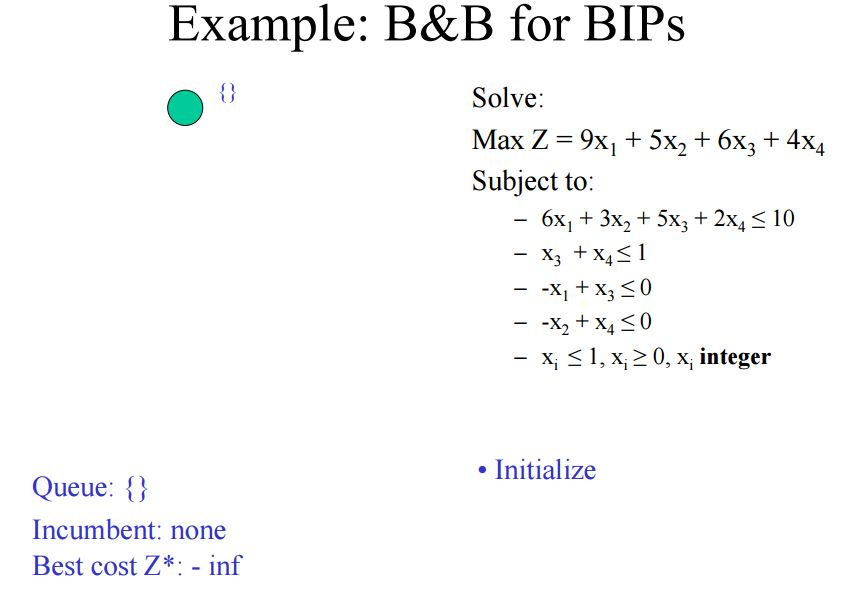
\includegraphics[width=1.1\linewidth]{BB-BIP/BB-BIP1}
\end{figure}
\end{frame}
\begin{frame}
	\begin{figure}
		\centering
		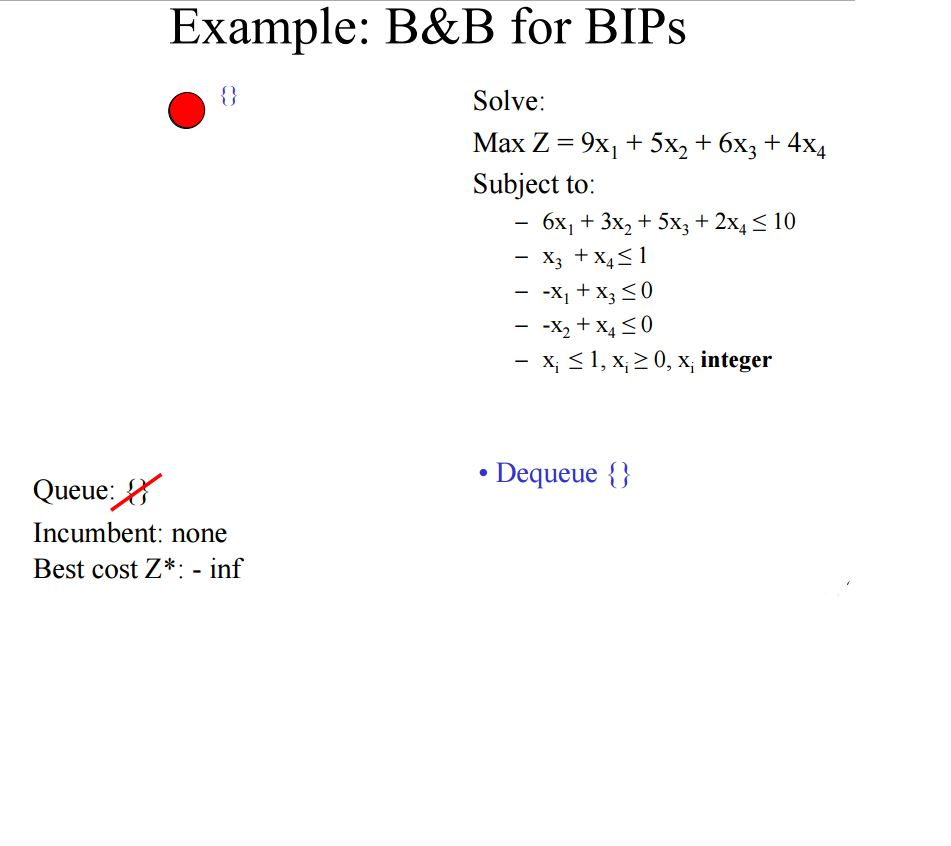
\includegraphics[width=1.1\linewidth]{BB-BIP/BB-BIP2}
	\end{figure}
\end{frame}
\begin{frame}
	\begin{figure}
		\centering
		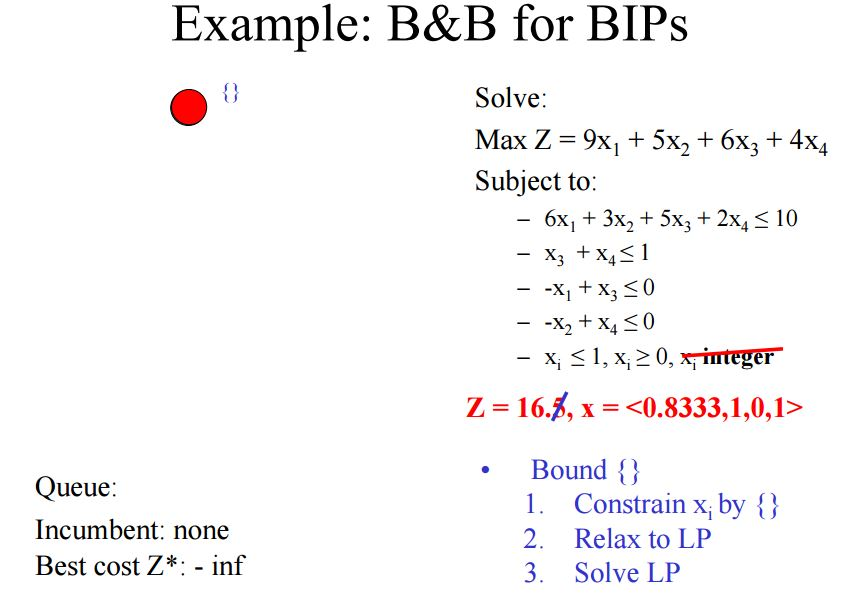
\includegraphics[width=1.0\linewidth]{BB-BIP/BB-BIP3}
	\end{figure}
\end{frame}
\begin{frame}
	\begin{figure}
		\centering
		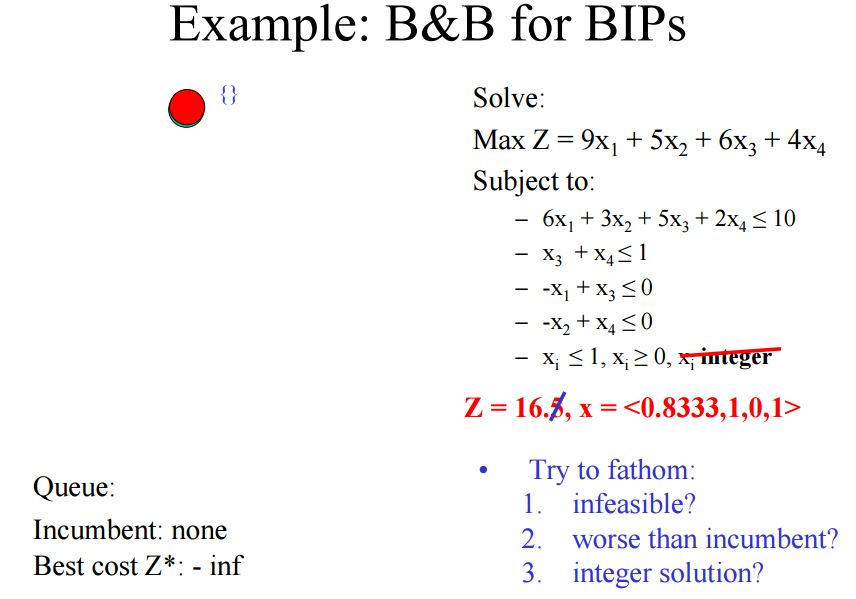
\includegraphics[width=1.0\linewidth]{BB-BIP/BB-BIP4}
	\end{figure}
\end{frame}

\begin{frame}
	\begin{figure}
		\centering
		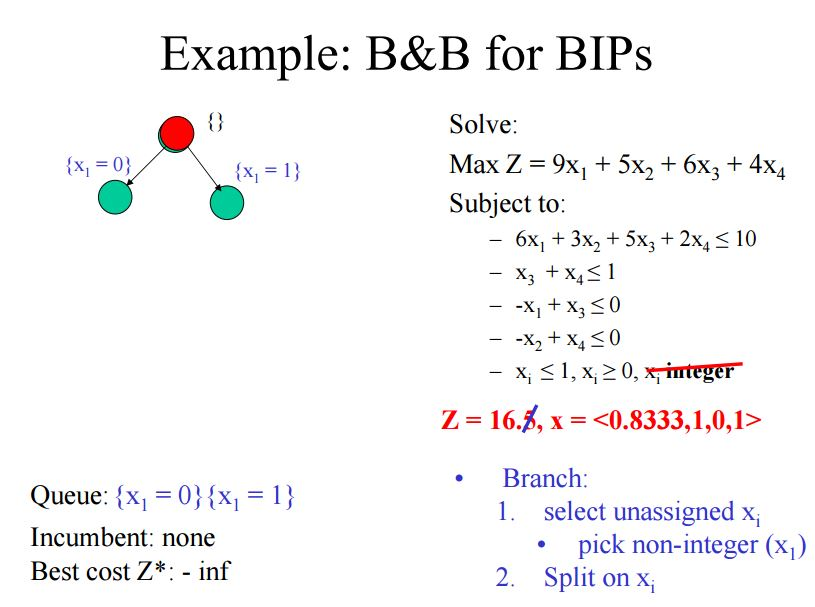
\includegraphics[width=1.1\linewidth]{BB-BIP/BB-BIP5}
	\end{figure}
\end{frame}
\begin{frame}
	\begin{figure}
		\centering
		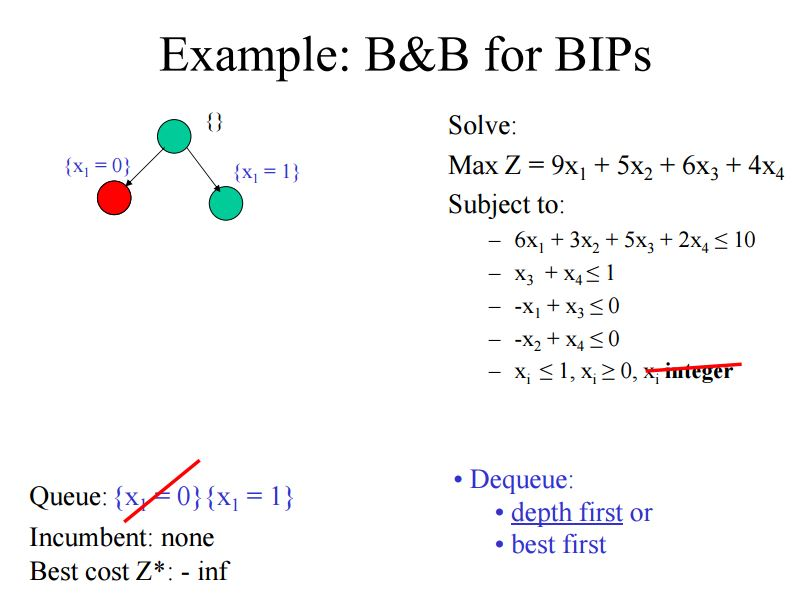
\includegraphics[width=1.0\linewidth]{BB-BIP/BB-BIP6}
	\end{figure}
\end{frame}
\begin{frame}
	\begin{figure}
		\centering
		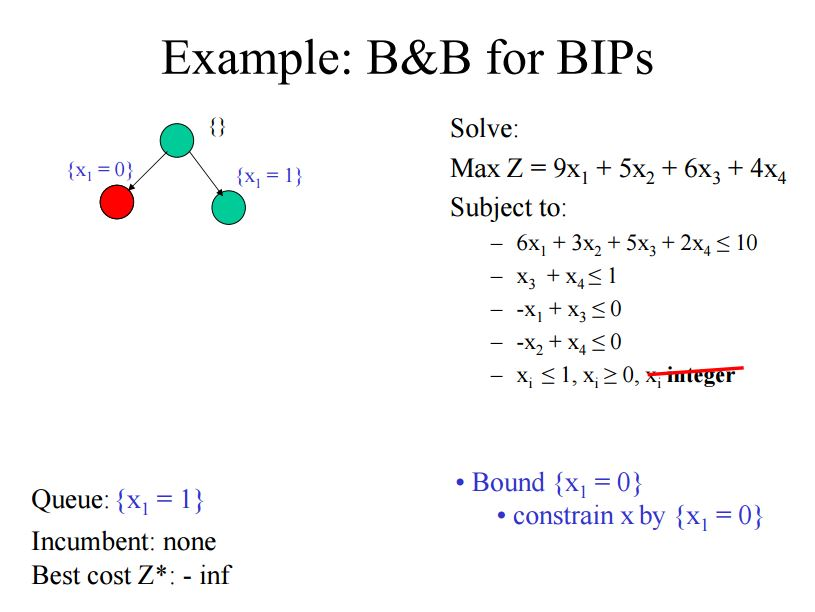
\includegraphics[width=1.0\linewidth]{BB-BIP/BB-BIP7}
	\end{figure}
\end{frame}
\begin{frame}
	\begin{figure}
		\centering
		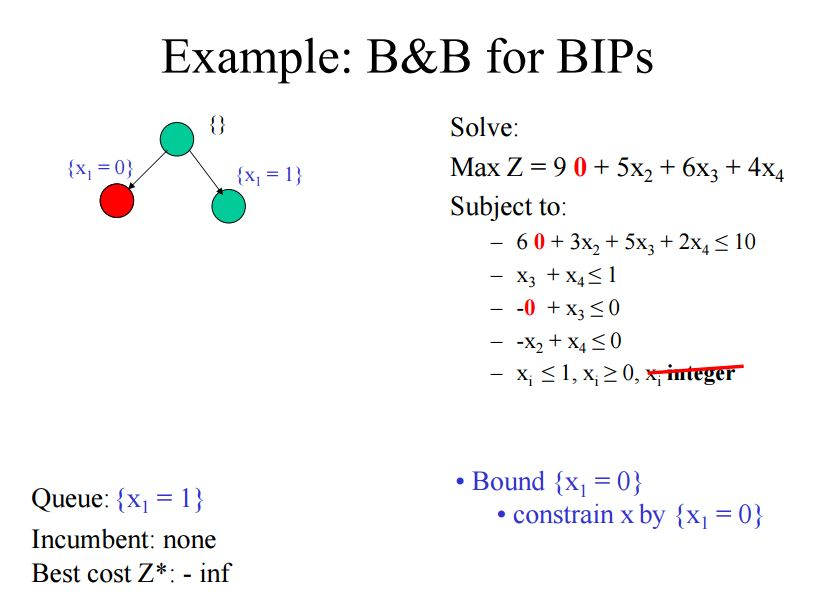
\includegraphics[width=1.1\linewidth]{BB-BIP/BB-BIP8}
	\end{figure}
\end{frame}
\begin{frame}
	\begin{figure}
		\centering
		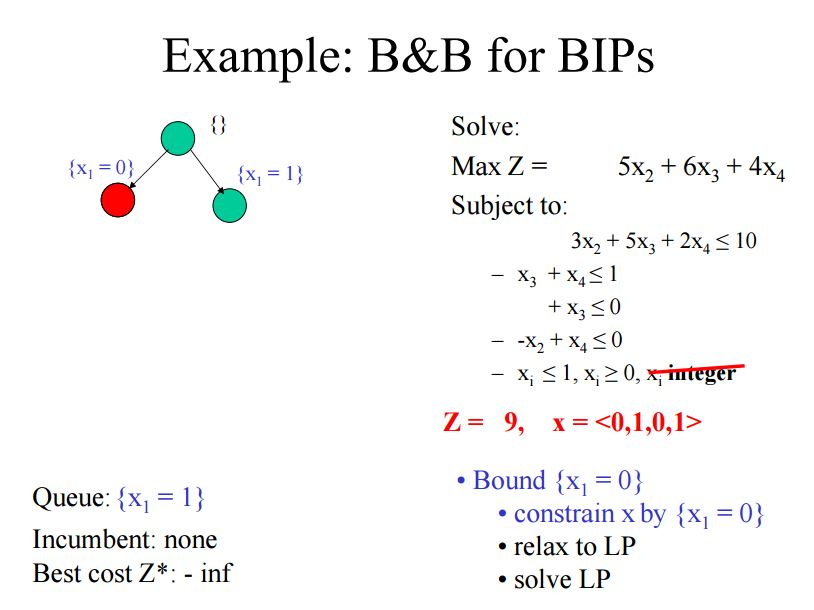
\includegraphics[width=1.0\linewidth]{BB-BIP/BB-BIP9}
	\end{figure}
\end{frame}
\begin{frame}
	\begin{figure}
		\centering
		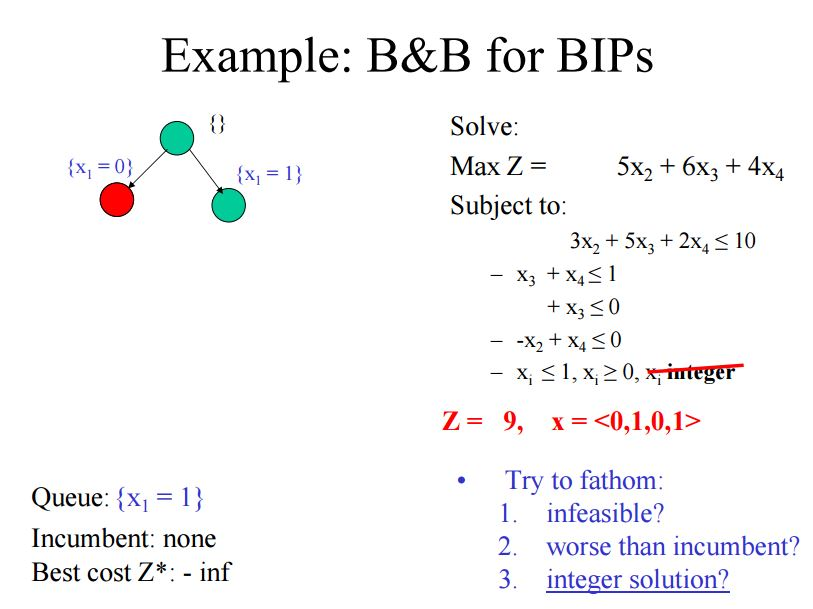
\includegraphics[width=1.0\linewidth]{BB-BIP/BB-BIP10}
	\end{figure}
\end{frame}
\begin{frame}
	\begin{figure}
		\centering
		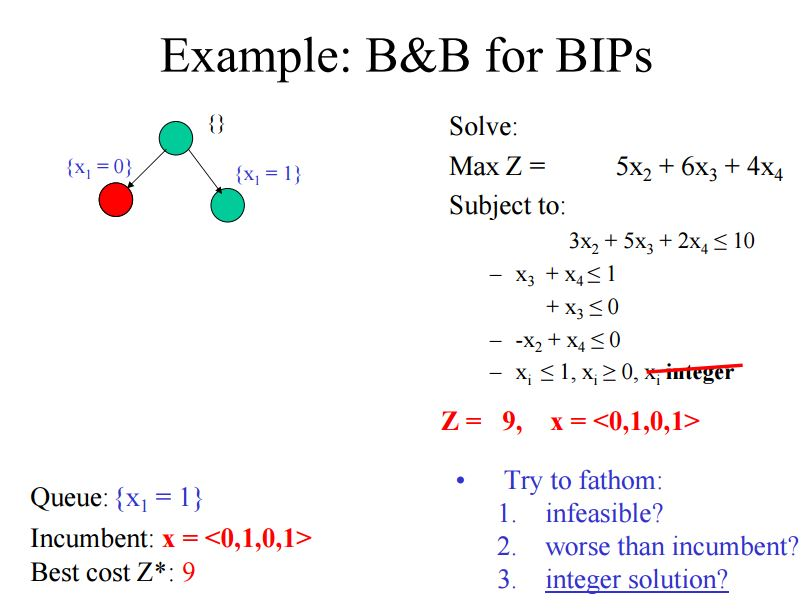
\includegraphics[width=1.0\linewidth]{BB-BIP/BB-BIP11}
	\end{figure}
\end{frame}
\begin{frame}
	\begin{figure}
		\centering
		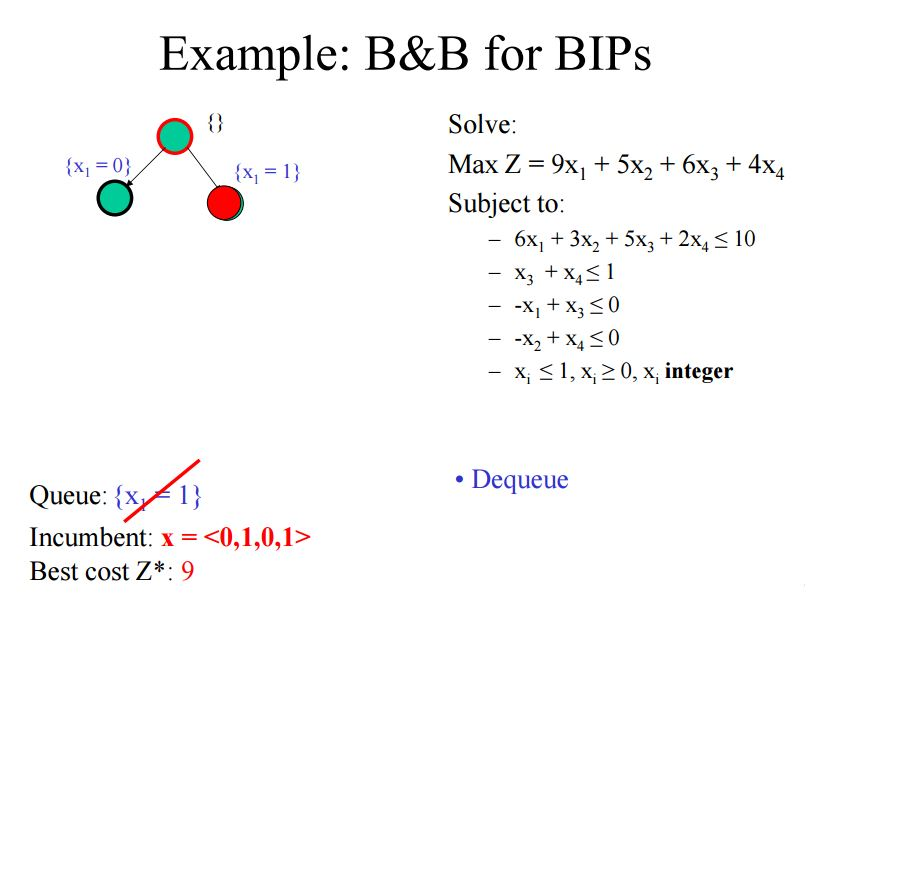
\includegraphics[width=1.1\linewidth]{BB-BIP/BB-BIP12}
	\end{figure}
\end{frame}
\begin{frame}
	\begin{figure}
		\centering
		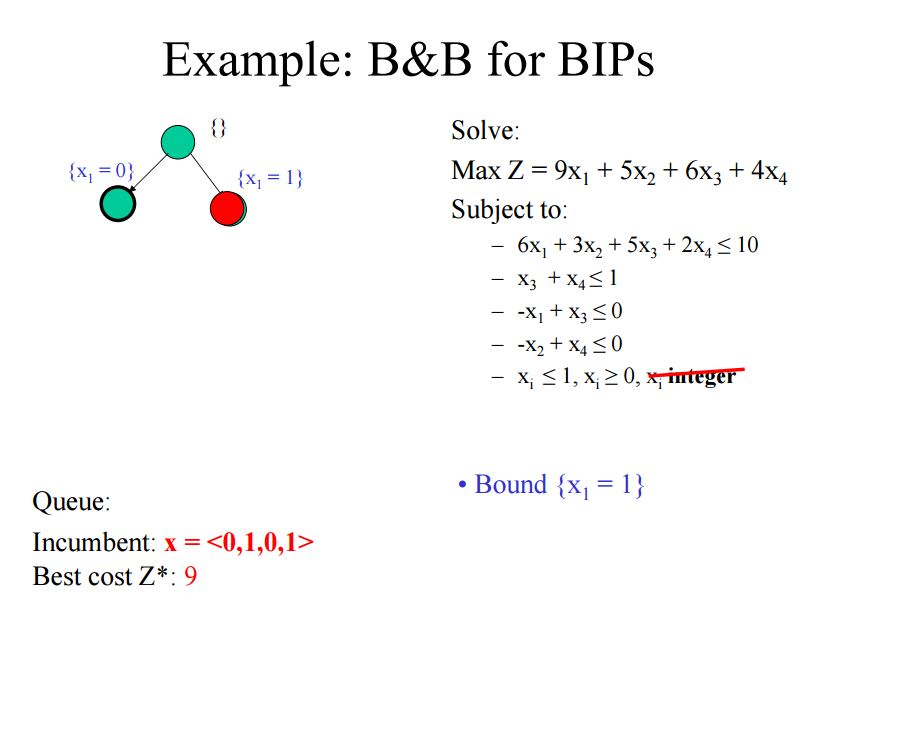
\includegraphics[width=1.0\linewidth]{BB-BIP/BB-BIP13}
	\end{figure}
\end{frame}
\begin{frame}
	\begin{figure}
		\centering
		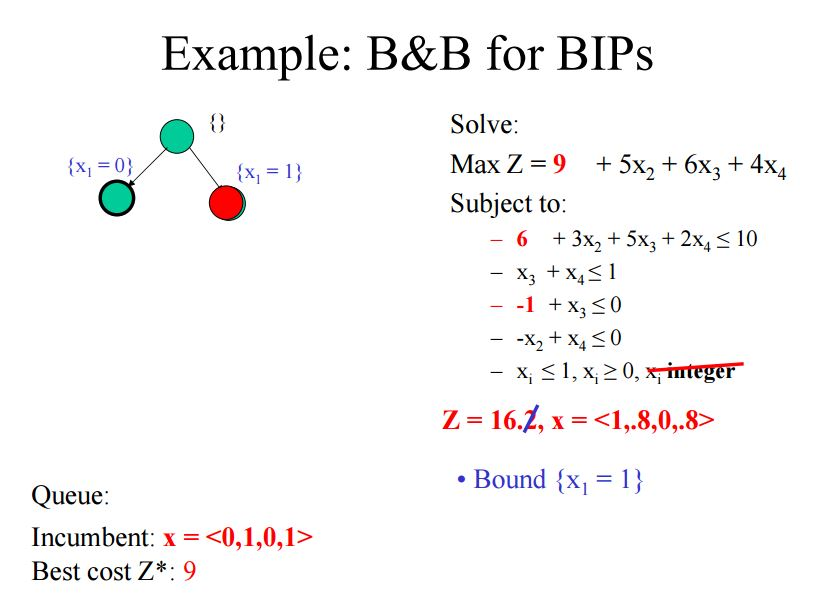
\includegraphics[width=1.0\linewidth]{BB-BIP/BB-BIP14}
	\end{figure}
\end{frame}
\begin{frame}
	\begin{figure}
		\centering
		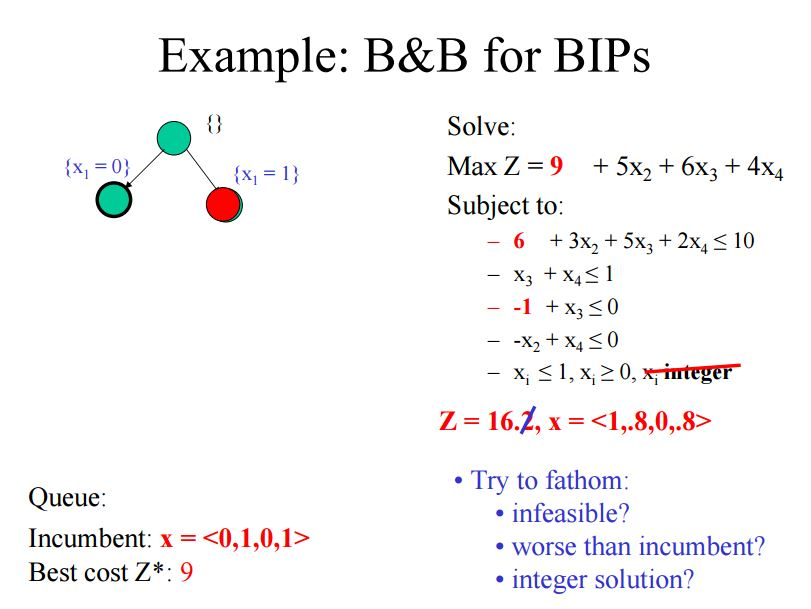
\includegraphics[width=1.0\linewidth]{BB-BIP/BB-BIP15}
	\end{figure}
\end{frame}
\begin{frame}
	\begin{figure}
		\centering
		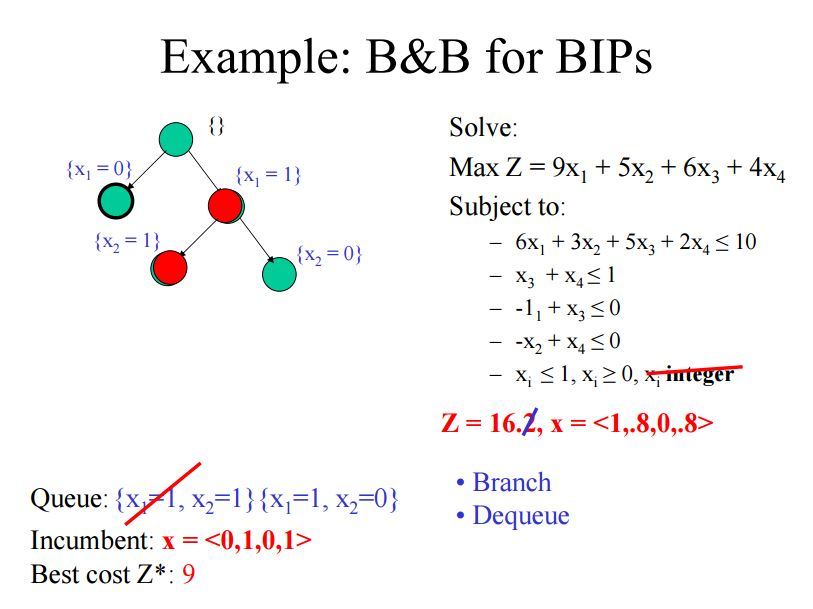
\includegraphics[width=1.1\linewidth]{BB-BIP/BB-BIP16}
	\end{figure}
\end{frame}
\begin{frame}
	\begin{figure}
		\centering
		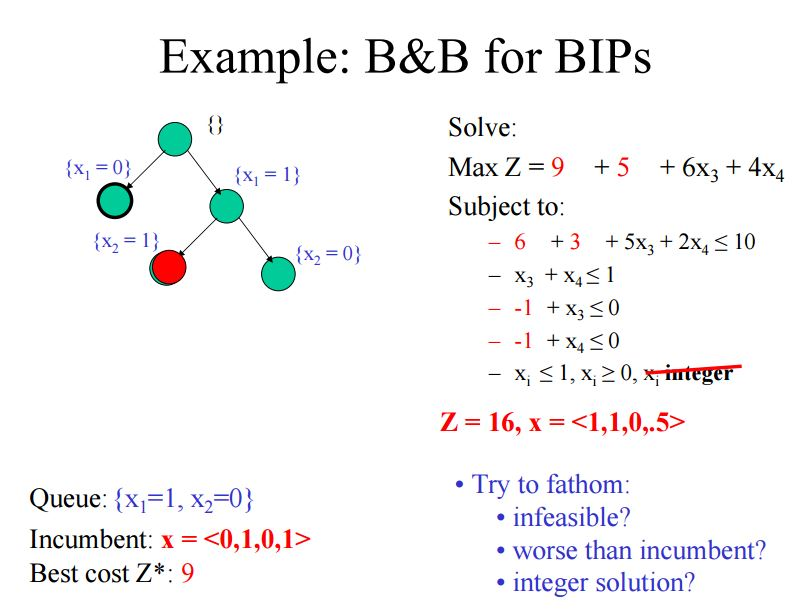
\includegraphics[width=1.0\linewidth]{BB-BIP/BB-BIP17}
	\end{figure}
\end{frame}
\begin{frame}
	\begin{figure}
		\centering
		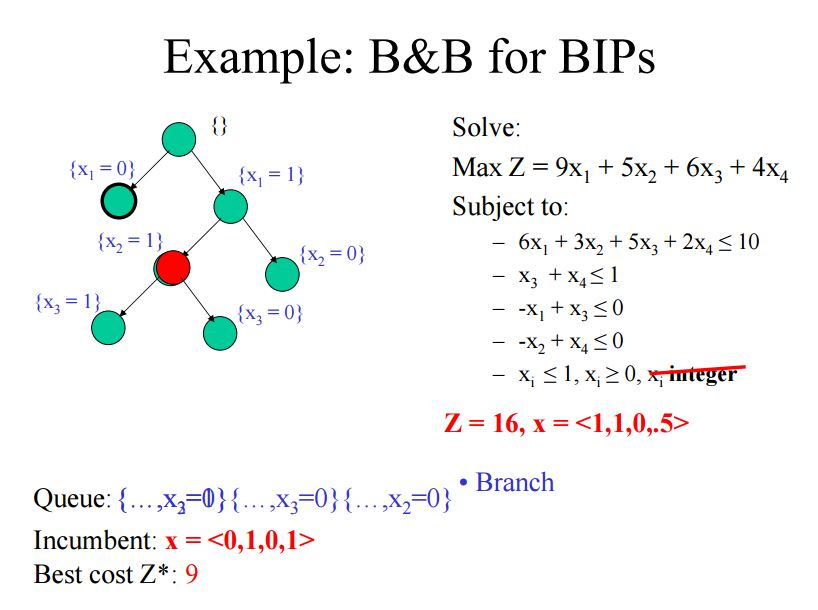
\includegraphics[width=1.0\linewidth]{BB-BIP/BB-BIP18}
	\end{figure}
\end{frame}
\begin{frame}
	\begin{figure}
		\centering
		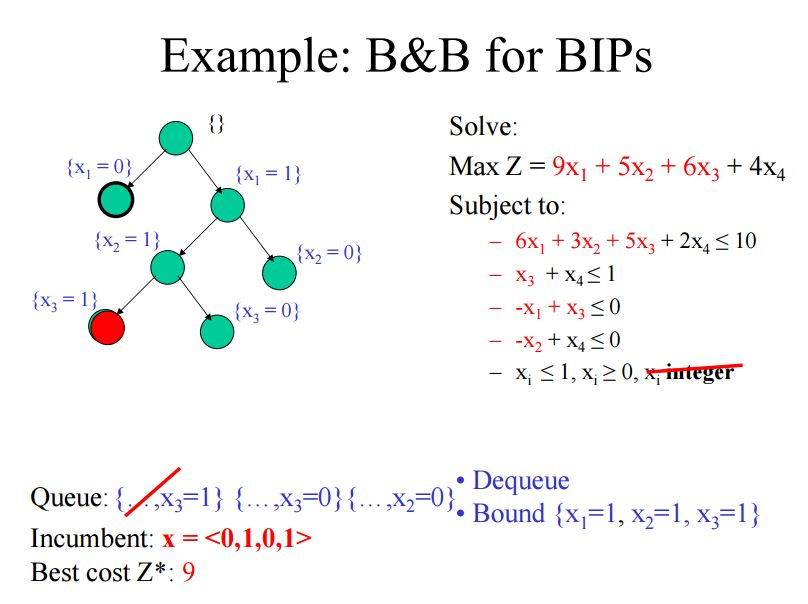
\includegraphics[width=1.0\linewidth]{BB-BIP/BB-BIP19}
	\end{figure}
\end{frame}
\begin{frame}
	\begin{figure}
		\centering
		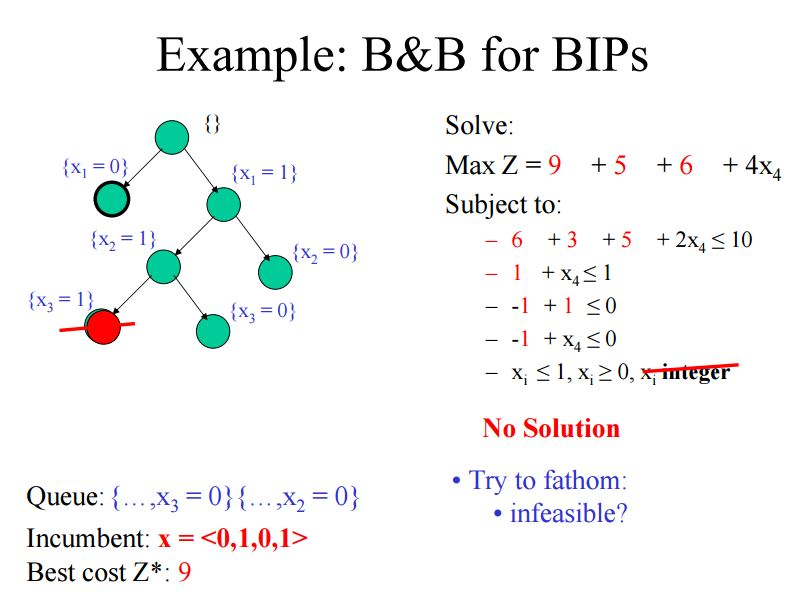
\includegraphics[width=1.1\linewidth]{BB-BIP/BB-BIP20}
	\end{figure}
\end{frame}
\begin{frame}
	\begin{figure}
		\centering
		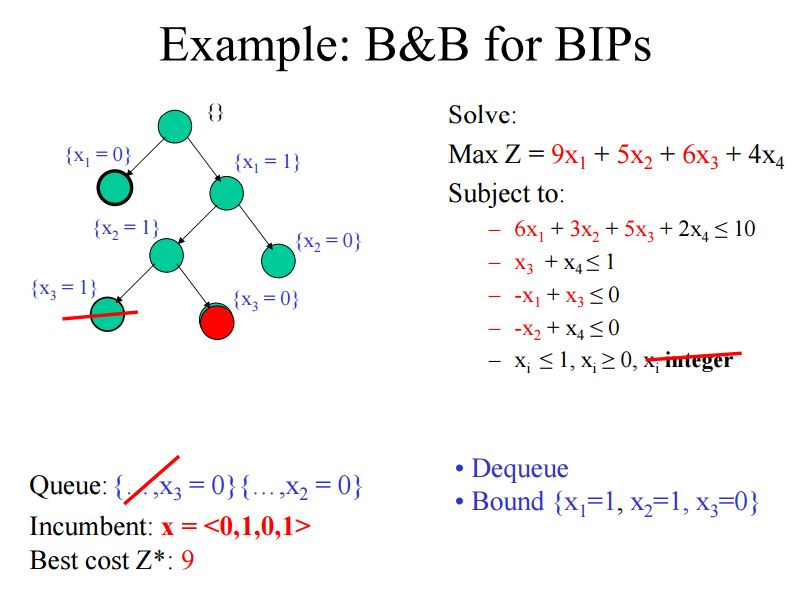
\includegraphics[width=1.0\linewidth]{BB-BIP/BB-BIP21}
	\end{figure}
\end{frame}
\begin{frame}
	\begin{figure}
		\centering
		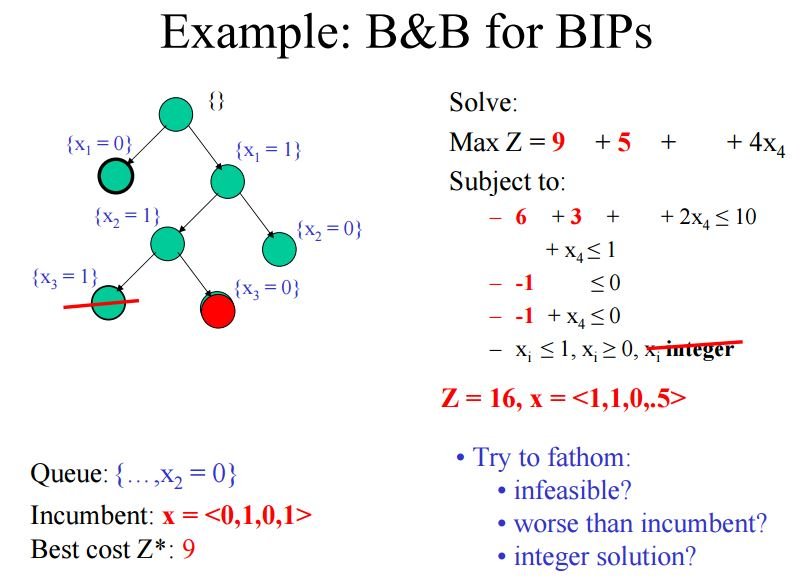
\includegraphics[width=1.0\linewidth]{BB-BIP/BB-BIP22}
	\end{figure}
\end{frame}
\begin{frame}
	\begin{figure}
		\centering
		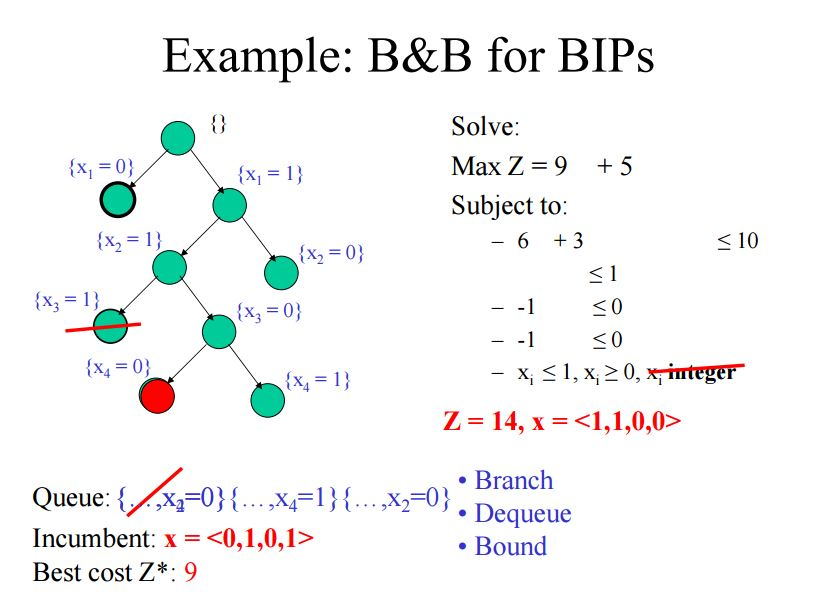
\includegraphics[width=1.0\linewidth]{BB-BIP/BB-BIP23}
	\end{figure}
\end{frame}
\begin{frame}
	\begin{figure}
		\centering
		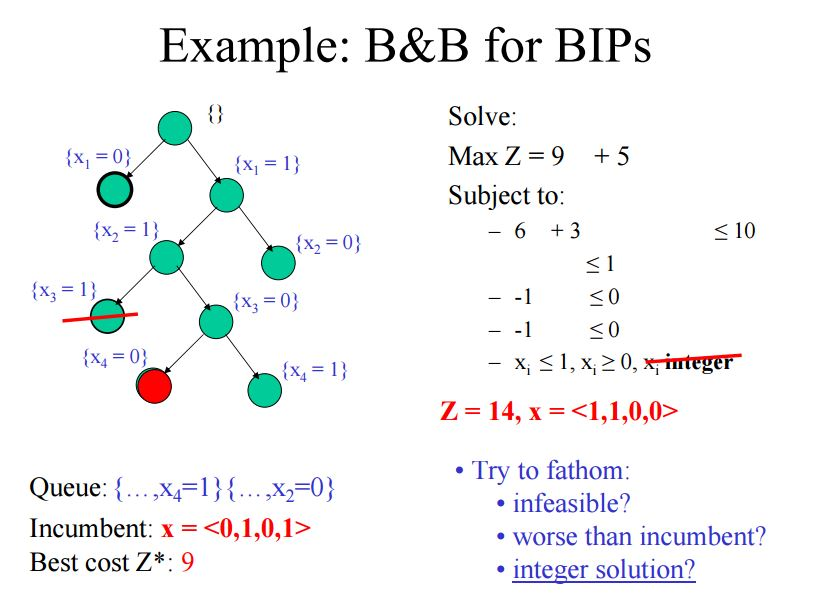
\includegraphics[width=1.1\linewidth]{BB-BIP/BB-BIP24}
	\end{figure}
\end{frame}
\begin{frame}
	\begin{figure}
		\centering
		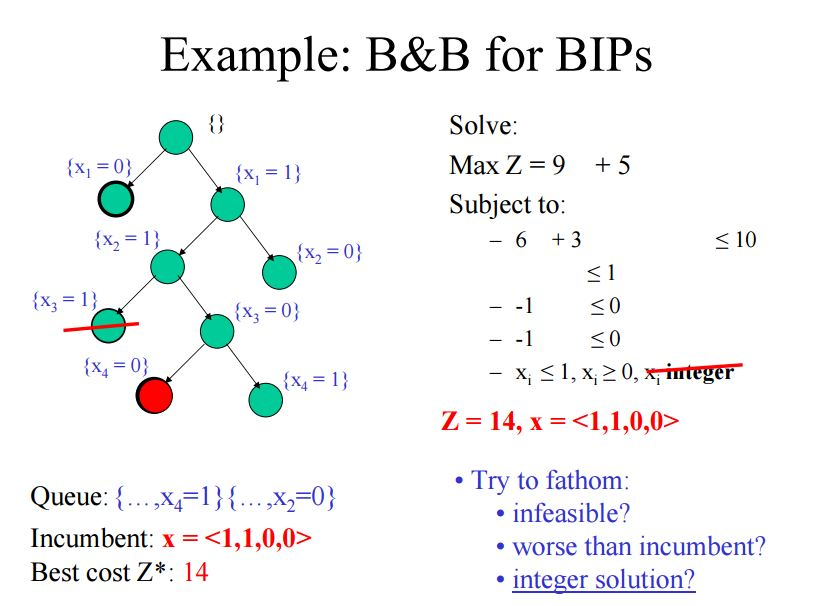
\includegraphics[width=1.0\linewidth]{BB-BIP/BB-BIP25}
	\end{figure}
\end{frame}
\begin{frame}
	\begin{figure}
		\centering
		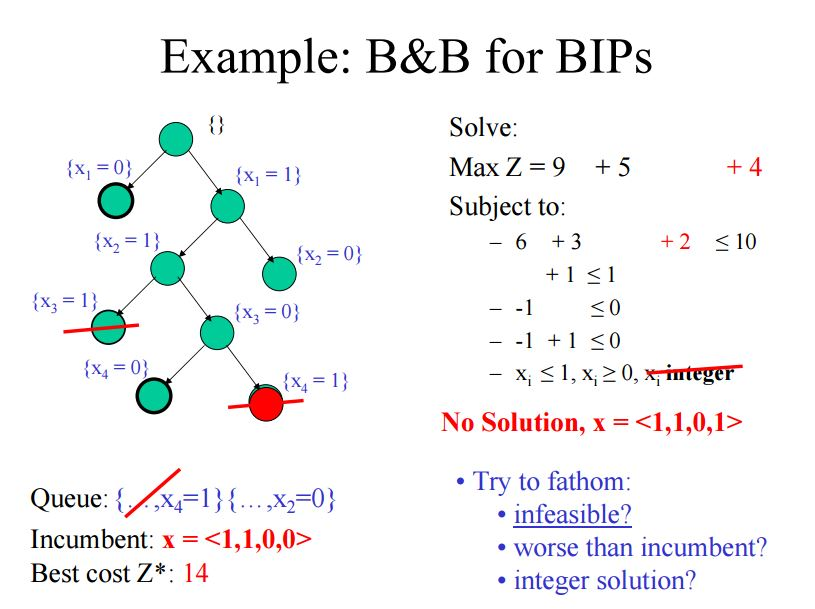
\includegraphics[width=1.0\linewidth]{BB-BIP/BB-BIP26}
	\end{figure}
\end{frame}
\begin{frame}
	\begin{figure}
		\centering
		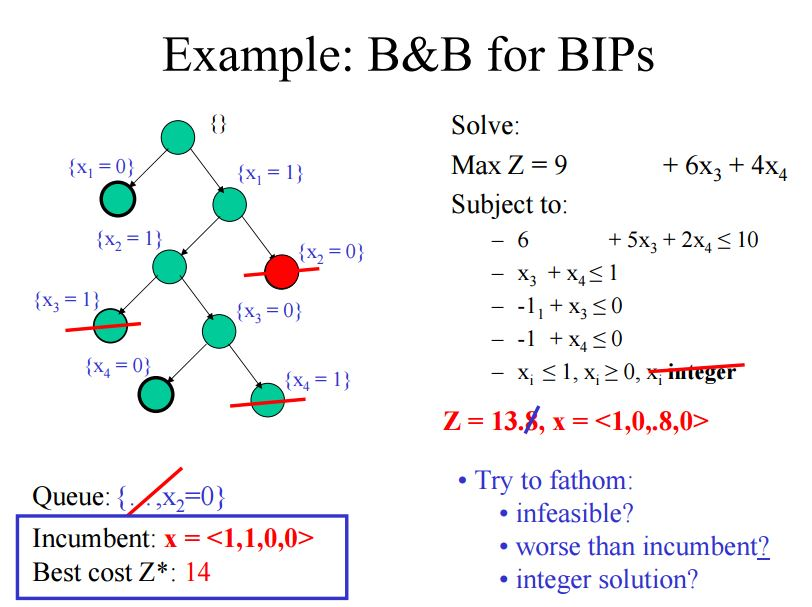
\includegraphics[width=1.0\linewidth]{BB-BIP/BB-BIP27}
	\end{figure}
\end{frame}
\end{document}
